\section{Definizione dell' architettura}
\subsection{Metodo e formalismo di specifica}
L' architettura del sistema è la struttura del sistema, che comprende gli elementi \textit{software}, la visibilità esterna di questi elementi e la relazione tra loro.
Questo documento andrà ad esporre le componenti di alto livello del sistema che verranno poi approfondite nel periodo di Progettazione di dettaglio e codifica, per analizzare l' architettura del sistema il \progetto si seguirà l' approccio \textit{top-down}, quindi innanzitutto si analizzerà il sistema fornendone una descrizione generale per poi scomporre le varie parti andando sempre più in dettaglio analizzando le singole componenti.
Successivamente si analizzeranno i \textit{design pattern} adottati e come verranno implementati.
Per esporre al meglio l architettura del sistema e il suo funzionamento di alto livello si utilizzeranno diagrammi dei \textit{package}, delle classi, di attività e di sequenza seguendo quanto imposto dalle \NormeDiProgetto{}.
\subsection{Architettura generale}
Il sistema \progetto{} è composto innanzitutto da due parti principali, un lato \textit{Client} e un lato \textit{Server}, per la loro progettazione si è tenuto conto dei principi della \textbf{riusabilità} e del \textbf{basso accoppiamento}, quindi si cercherà di progettare le due parti distintamente e senza dipendenze mantenendo all' oscuro il funzionamento del \textbf{server} al \textbf{client} e viceversa.\\
Dopo un' attenta analisi si è deciso di adottare il \textit{design pattern} architetturale \textbf{MVP} seguendo la variante \textit{Passive View}. Tale scelta è stata fatta per i seguenti motivi:
\begin{itemize}
%490.317 visualizzazioni
	\item ottenere una \textit{view} priva di \textit{application logic} che verrà delegata al \textit{presenter}, questo semplificherà i test, infatti la vista sarà un semplice \textit{mockup} e il \textit{presenter} può essere testato separatamente dalla vista;
	\item offre un' architettura solida e mantenibile attraverso il disaccoppiamento massimo tra viste e modelli.
\end{itemize}
\subsubsection{Componente View}
Questa componente andrà a costituire la \textbf{GUI} del sistema e sarà divisa in due parti, lato amministratore e quello utente. Entrambe le parti non dovranno fare altro che offrire un' interfaccia agli utenti del sistema utilizzando HTML5, CSS e Javascript.
\subsubsection{Componente Presenter}
Il \textit{presenter} andrà a rappresentare la \textit{application logic} del sistema e sarà divisa tra il lato Server e il lato Client. Le funzionalità che andrà a ricoprire saranno:
\begin{itemize}
	\item gestire parte della comunicazione tra le due parti;
	\item acquisire i dati inseriti dagli utenti ed elaborarli;
	\item mantenere aggiornata la vista in modo che rifletta i cambiamenti del model.
\end{itemize}
La maggior parte delle funzionalità saranno ricoperte dal \textit{presenter} lato \textit{client}, in quanto sarà responsabile di:
\begin{itemize}
	\item aggiornare le viste dell' utente e dell' amministratore;
	\item controllare i dati inseriti dall' utente e quando possibile elaborarli;
	\item passare i dati che necessitano di elaborazione lato \textit{server} al \textit{presenter} dello stesso;
	\item ricevere le risposte dal lato \textit{server} e fornire all' utente la vista aggiornata.
\end{itemize}
I ruoli del \textit{presenter} lato \textit{server} sono:
\begin{itemize}
 \item ricevere le richieste dal \textit{presenter} lato \textit{client} ed elaborarle, restituendo poi il risultato sotto forma di \textbf{JSON};
 \item informare il lato client delle modifiche effettuate sul model.
\end{itemize}
\subsubsection{Componente Model}
Questa componente andrà a rappresentare la \textit{business logic} del sistema, e sarà suddivisa tra \textit{client} in minima parte e \textit{server}.
I ruoli del componente lato \textit{client} saranno di mantenere traccia dell' utente autenticato e di salvare, qualora si decida di implementare questa funzionalità, i dati come per esempio coordinate gps e immagini quando il dispositivo non disporrà di connessione internet.

\begin{figure}[H] \centering 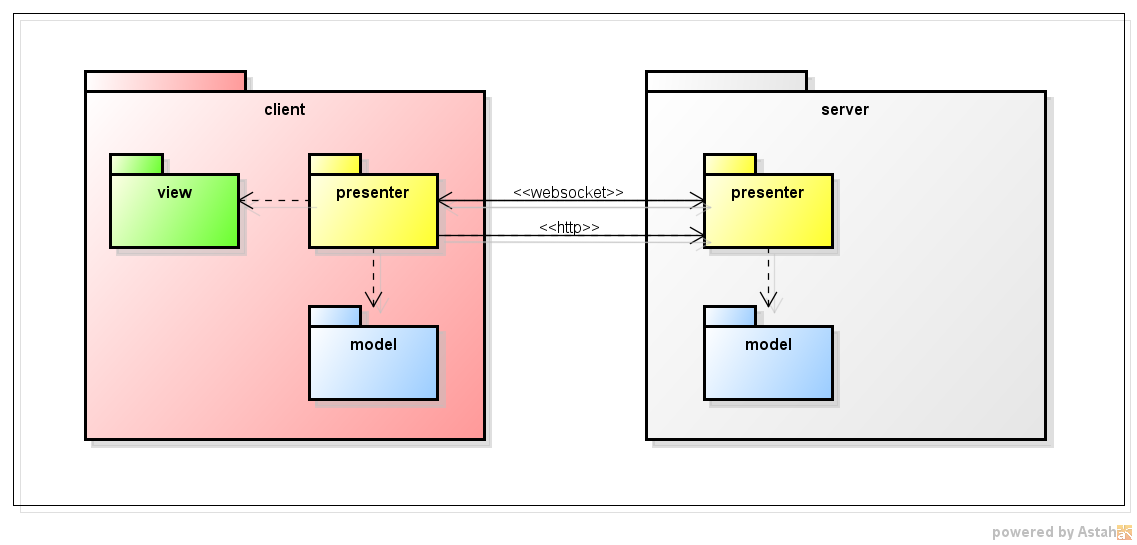
\includegraphics[width=%
\textwidth]
{./other/MVPIntroduzione.png} \caption{Diagramma UML architettura generale}
\end{figure}